\documentclass[12p, a4paper, onecolumn]{report} 
\usepackage[utf8x]{inputenc} 
\usepackage[T1]{fontenc}
\usepackage[english]{babel} % replace with serbian later
\usepackage[vmargin=20mm, hmargin=25mm]{geometry}
\usepackage[ampersand]{easylist}
\usepackage[PetersLenny]{fncychap} % Sonny, Lenny, Glenn, Conny, Rejne, Bjarne, PetersLenny, Bjornstrup
\usepackage[colorlinks=true, linkcolor=black, citecolor=green, filecolor=magenta, urlcolor=cyan]{hyperref}

%\usepackage{algorithm}
\usepackage[lined,boxed,commentsnumbered]{algorithm2e}
\usepackage{algorithmic}
%\usepackage{algpseudocode}
\usepackage{amsbsy}
\usepackage{amsfonts}
\usepackage{amsmath}
\usepackage{amssymb}
\usepackage{amsthm}
\usepackage{appendix}
\usepackage{caption}
\usepackage{color} 
\usepackage{empheq}
\usepackage{etoolbox}
\usepackage{fancyhdr}
\usepackage{float}
\usepackage{graphicx}
\usepackage{latexsym}
\usepackage{leftidx}
\usepackage{lipsum}
\usepackage{listings}
\usepackage{lmodern}
\usepackage{mathtools}
\usepackage{multicol}
\usepackage{newlfont}
\usepackage{slantsc}
\usepackage{tikz}
\usepackage{titlesec}

\usetikzlibrary{arrows,decorations.pathmorphing,backgrounds,positioning,fit,petri}
\usetikzlibrary{shapes.geometric}

\tikzset{
    triangle/.style={
        draw,
        shape border rotate=0,
        regular polygon,
        regular polygon sides=3,
        fill=white,
        node distance=2cm,
        minimum height=4em,
        minimum size=4mm,
        inner sep=0pt
    }
}

\renewcommand*{\algorithmcfname}{\cyb Algoritam}% Algorithm name

% C++ Code
\definecolor{mygreen}{rgb}{0,0.6,0}
\definecolor{mygray}{rgb}{0.5,0.5,0.5}
\definecolor{mymauve}{rgb}{0.58,0,0.82}

\lstset{ %
  backgroundcolor=\color{white},   % choose the background color; you must add \usepackage{color} or \usepackage{xcolor}
  basicstyle=\footnotesize,        % the size of the fonts that are used for the code
  breakatwhitespace=false,         % sets if automatic breaks should only happen at whitespace
  breaklines=true,                 % sets automatic line breaking
  captionpos=b,                    % sets the caption-position to bottom
  commentstyle=\color{mygreen},    % comment style
  deletekeywords={...},            % if you want to delete keywords from the given language
  escapeinside={\%*}{*)},          % if you want to add LaTeX within your code
  extendedchars=true,              % lets you use non-ASCII characters; for 8-bits encodings only, does not work with UTF-8
  frame=false,                    % adds a frame around the code
  keepspaces=true,                 % keeps spaces in text, useful for keeping indentation of code (possibly needs columns=flexible)
  keywordstyle=\color{blue},       % keyword style
  language=C++,                 % the language of the code
  morekeywords={*,...},            % if you want to add more keywords to the set
  numbers=left,                    % where to put the line-numbers; possible values are (none, left, right)
  numbersep=5pt,                   % how far the line-numbers are from the code
  numberstyle=\tiny\color{mygray}, % the style that is used for the line-numbers
  rulecolor=\color{black},         % if not set, the frame-color may be changed on line-breaks within not-black text (e.g. comments (green here))
  showspaces=false,                % show spaces everywhere adding particular underscores; it overrides 'showstringspaces'
  showstringspaces=false,          % underline spaces within strings only
  showtabs=false,                  % show tabs within strings adding particular underscores
  stepnumber=1,                    % the step between two line-numbers. If it's 1, each line will be numbered
  stringstyle=\color{mymauve},     % string literal style
  tabsize=2,                       % sets default tabsize to 2 spaces
  title=\lstname                   % show the filename of files included with \lstinputlisting; also try caption instead of title
}

% Cyrillic font

% dj, zh, lj, nj, c1, ch, d2, sh
% \/ (backslash-forwardslash) to split

\font \cyrtitle=wncyr10 at 18pt
\font \cyrsubtitle=wncyr10 at 12pt
\font \cyrsection=wncyb10 at 13pt
\font \cyr=wncyr10 at 11pt
\font \cyi=wncyi10 at 11pt
\font \cyb=wncyb10 at 11pt

\captionsetup[algorithm]{name={\cyr Algoritam}}
\captionsetup[figure]{labelfont=bf}

\makeatletter
\titleformat{\chapter}[frame]
  {\normalfont}{\filright\enspace \@chapapp~\thechapter\enspace}
  {8pt}{\LARGE\bfseries\filcenter}
\titlespacing*{\chapter}
  {0pt}{0pt}{20pt}

\makeatother

\definecolor{gray75}{gray}{0.75}
\newcommand{\hsp}{\hspace{20pt}}
\titleformat{\chapter}[hang]{\Huge\bfseries}{\thechapter\hsp\textcolor{gray75}{|}\hsp}{0pt}{\Huge\bfseries}

\pagestyle{fancy}
\renewcommand{\headrulewidth}{0pt}
\renewcommand{\footrulewidth}{0pt}
\lhead{\textsl{\textsc{Group Project Team Echo}}}
\rhead{\textsl{\textsc{Multi-touch Conference}}}

\fancypagestyle{plain}{ % remove everything
  \renewcommand{\headrulewidth}{0pt} % remove lines as well
  \renewcommand{\footrulewidth}{0pt}}
  
\setcounter{secnumdepth}{4}
\setcounter{tocdepth}{4}

\begin{document}

\begin{titlepage}

\newcommand{\HRule}{\rule{\linewidth}{0.5mm}} % Defines a new command for the horizontal lines, change thickness here
\clearpage
\vspace*{\fill}
\center % Center everything on the page
 
%----------------------------------------------------------------------------------------
%	HEADING SECTIONS
%----------------------------------------------------------------------------------------

\textsc{\LARGE University of Cambridge}\\[1.5cm] % Name of your university/college
\textsc{\Large Computer Science Tripos, Part IB}\\[0.5cm] % Major heading such as course name
\textsc{\large Group Project Team Echo}\\[0.5cm] % Minor heading such as course title

%----------------------------------------------------------------------------------------
%	TITLE SECTION
%----------------------------------------------------------------------------------------

\HRule \\[0.4cm]
{ \huge \bfseries Multi-touch Conference}\\[0.4cm]
{ \huge \bfseries Project plan}\\[0.1cm] % Title of your document
\HRule \\[1.5cm]
 
%----------------------------------------------------------------------------------------
%	AUTHOR SECTION
%----------------------------------------------------------------------------------------

\begin{minipage}{0.4\textwidth}
\begin{flushleft} \large
\emph{Authors:}\\
Mona Niknafs (\texttt{mn407})\\
Yojan Patel (\texttt{yp242})\\
Alexandru Tache (\texttt{at628})\\
Philip Thomson (\texttt{prt28})\\
Petar Veli\v{c}kovi\'{c} (\texttt{pv273})\\
\end{flushleft}
\end{minipage}
~
\begin{minipage}{0.4\textwidth}
\begin{flushright} \large
\emph{Client:} \\
Catherine White, BT\\ 
\hfill \\
\hfill \\
\hfill \\
\hfill \\
\end{flushright}
\end{minipage}\\[4cm]

%----------------------------------------------------------------------------------------
%	DATE SECTION
%----------------------------------------------------------------------------------------

{\large 28 January 2014}\\[3cm] % Date, change the \today to a set date if you want to be precise

%----------------------------------------------------------------------------------------
%	LOGO SECTION
%----------------------------------------------------------------------------------------


\includegraphics{logo.png}\\[1cm] % Include a department/university logo - this will require the graphicx package
 
%----------------------------------------------------------------------------------------

\vfill % Fill the rest of the page with whitespace

\end{titlepage}

\setcounter{page}{1}
\pagenumbering{roman}

\tableofcontents

\newpage

\setcounter{page}{1}
\pagenumbering{arabic}

\chapter{Project Plan}

\section{Introduction}

The main purpose of this document is to present a more detailed breakdown of the technical work that is required to be undertaken for the Multi-touch Conference group project, as described in \emph{Appendix A} (Management Strategy) of the functional specification document. As most of the functionalities are already described in that document, the module descriptions here are brief, and more emphasis is given to the amount of people/time needed to implement them, testing strategies, and diagrams that will enhance the reader’s understanding of the module structures and dependencies. Note that the UML diagrams shown here will represent only the bare minimum of methods we would expect the listed classes to have; it is highly likely that the final project will have a different abstract class layout (which is still based upon the diagrams given here).

\section{Modules}

The project will be split in the following \textbf{five} modules:
\begin{itemize}
\item the server;
\item a client base library for communicating with the server, and its extensions:
\begin{itemize}
  \item the touchscreen client;
  \item the Android client;
  \item the computer client.
\end{itemize}
\end{itemize}
There is an additional package (the \emph{“data”} package) containing all the classes that represent units of data stored within or in movement between the other modules. This section describes each of those modules in turn, with accompanying UML diagrams to aid clarity.

\subsection{Server}

The \textbf{server} will be the core component of our project. It can be split into two large components: 
\begin{itemize}
\item a \textbf{client handler}, that handles and multiplexes all of the messages received from clients and produces appropriate replies to the relevant client(s);
\item a \textbf{data analyst}, that upon request processes conversation data in order to produce various kinds of output, f.ex. keywords for individual conversations, conversations sorted by popularity, searching for particular words, and many other possibilities. 
\end{itemize}
Since the server will store all the conference data it must be resilient to failure, thus all the data must be stored in a database on disk. A more detailed structure of the server is shown on \emph{Figure 1.1}. \\ \\
The server is the largest and hardest module to implement and as such \textbf{two} group members are assigned to work on it (with the work roughly split between the client handling and data analysis tools). Testing the client handler will involve stressing it with different kinds of client load scenarios and observing the response latency, and the data analyst will be tested by feeding pre-made conversation data (f.ex. scripts from movies) and observing the usefulness of the output (f.ex. whether or not the keywords extracted correspond to the movie’s theme, etc).
The entire work regarding implementing and testing the server should not take more than 30h/person, if no major difficulties arise.
\begin{figure}[H]
  \centering
  \includegraphics[width=\textwidth]{UMLServer.jpg}
  \caption{UML diagram depicting a more detailed structure of the server.}
\end{figure}

\subsection{Client}

In order for other modules to easily operate with the server, a \textbf{client library} that handles all the server communication needs to be provided. Its structure is relatively simple, because it only serves to provide all the clients a single type of base class that will directly contact the server on their behalf (this involves implementing methods for sending and receiving messages to/from the server and handling basic events); all the additional interesting processing of the received raw data from the server is handled in the modules that extend it. Because of that, we anticipate that the base client should be a simple module to implement and as such, only \textbf{one} person is assigned to its implementation. It should not take more than 5h of work to have a stable implementation, and testing will be performed in conjunction with the server.

\begin{figure}[H]
  \centering
  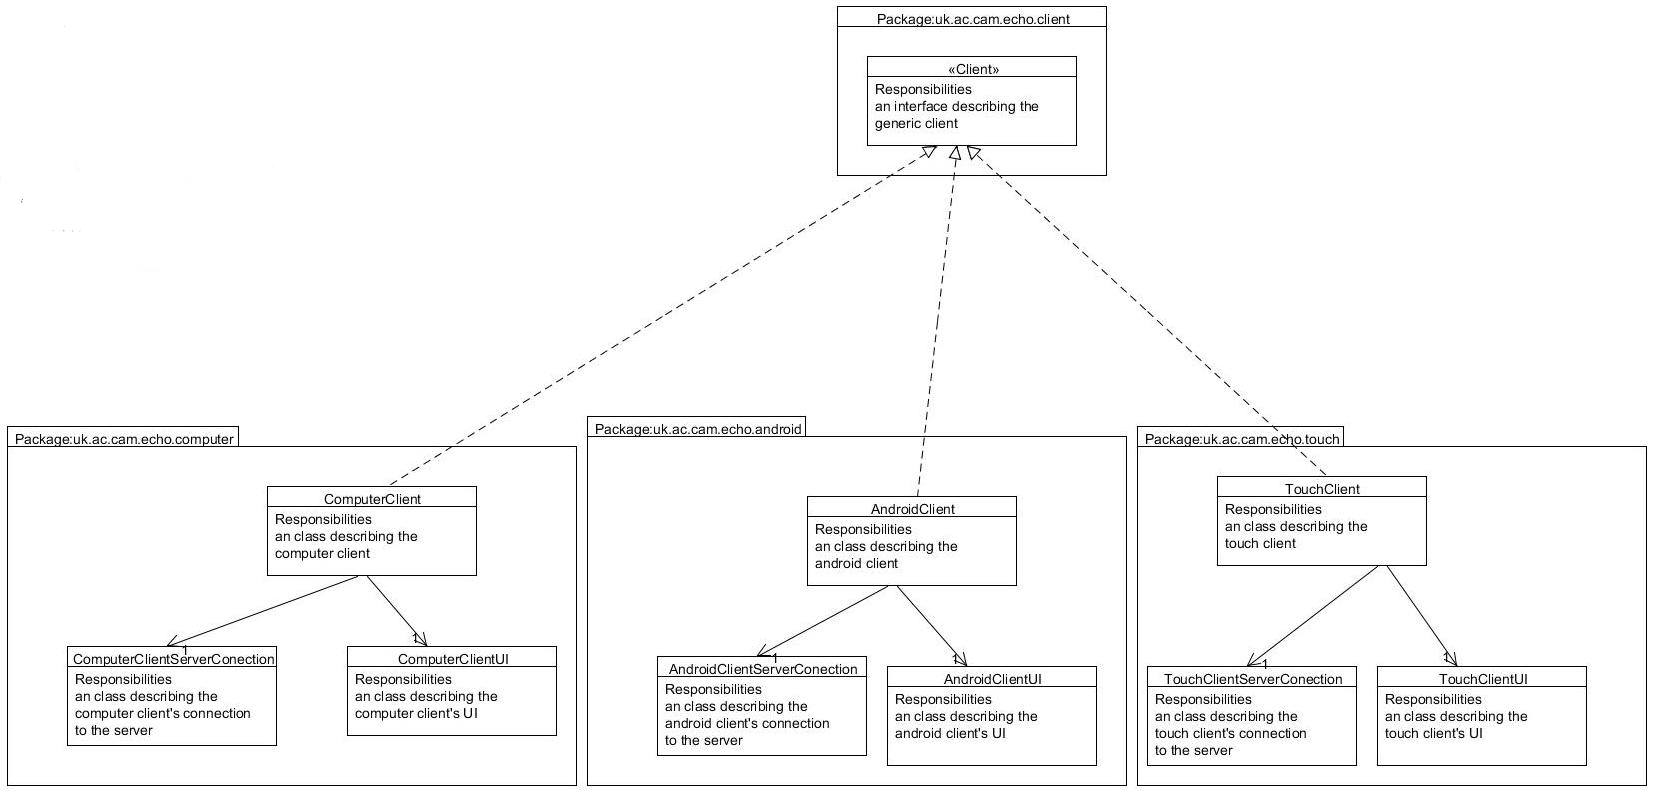
\includegraphics[width=0.955\textwidth]{UMLClient.jpg}
  \caption{UML diagram depicting a more detailed structure of the client and its extensions.}
\end{figure}

\subsubsection{Touchscreen client}

The \textbf{touchscreen client} will be the main user interface. The application will run on a PC running Windows 8.1, with a 27+ inch multi-touch screen that supports at least 10 simultaneous touches. Its role will be to allow multiple users to follow and contribute to different conversations simultaneously using the touch capabilities of the screen. It should also provide users with suggestions about other relevant conversations they might be interested in joining, as well as personalised information for the users that are currently connected with the screen. As part of this effort the application will need to communicate with the server using the library specified in subsection 1.2.2, and interpret the received data to provide useful output for the users; also, it should be able to generate QR codes that the client mobile applications will be able to scan in order to connect to a specific conversation. \\ \\
This module clearly has the largest demonstrative value, as its proper implementation will display exactly how a multi-touch screen can enhance the conferencing experience, which is the key distinctive feature of this project. It is also the module where we expect the most implementation challenges, depending on how many problems arise from the touchscreen API. To reflect its importance and possible difficulties, \textbf{two} group members will be assigned to the implementation this module at all times, with additional members joining in for assistance as needed. Tests will involve issuing different kinds of request batches to the server and observing the output, as well as scheduling “mock conferences” among group members in order to investigate its conference-enhancing value. We estimate this module to require roughly up to 30h of work per person, however this is subject to change.

\subsubsection{Android client}

The \textbf{Android client} will be implemented as an application that will provide a simple interface that will enable individuals to contribute to group conversations using their personal smartphone/tablet devices. As the touchscreen client the application should use the library from subsection 1.2.2 in order to communicate messages and requests to the server. It should periodically display notifications to the user about interesting topics, give suggestions for conversations to join, allow for keyword/tag searching of conversations, and enable QR code scanning to integrate with the multi-touch screen’s interface if desired. \\ \\
This is a very important module as it will likely be the dominant manner of communication between users in most scenarios, however its implementation should be fairly straightforward, as well as testing (as there are only a handful of features to test, and they can be done by running the application on any Android smartphone/tablet and observing the behaviour). Hence only \textbf{one} group member will be assigned to work on this module and a reasonably stable application should be expected within 20h of work.

\subsubsection{Computer client}

As an additional extension, we will implement a \textbf{computer client} that is designed to run on a PC with a generic monitor without touchscreen capabilities. Using a personal computer during a conference falls out of the usage model we have predicted for this application, and we have opted to design it solely for the purpose of an additional means of testing the final product. As such its interface will be minimal, with controlling the application and receiving the output done either via the terminal or with a very simple graphical interface. \textbf{One} group member is assigned to this module, and we expect it in a stable state within 3h of work.

\subsection{Data}

This package contains all the various kinds of \textbf{custom data classes} that satisfy any of the following criteria:
\begin{itemize}
\item are stored within any of the modules;
\item are transferred between modules in any way (f.ex. for message passing);
\item are stored in the server database and can be queried upon.
\end{itemize}
\begin{figure}[h]
  \centering
  \includegraphics[width=\textwidth]{UMLData.jpg}
  \caption{UML diagram depicting a more detailed structure of the data package.}
\end{figure}
We have initially identified a few essential data classes that are bound to be used in multiple modules (such as User, Message, Conversation, Conference…) and it is likely that more classes will be added as development proceeds. As the need for these classes arises during development, no particular group member is assigned to implement this part; whoever discovers the need for a new data class will be assumed responsible to provide at least an interface that the remainder of the group can use, and if possible an implementation. The data will be modeled to be \textbf{persistent} and easily \textbf{storable} in a database.

\section{Module dependencies}

All modules described above are dependent on the “data” package to provide a unanimous representation of data within the project; otherwise:
\begin{itemize}
\item the server will have no dependencies;
\item the client library will depend on the server implementation (determining the manner in which the client must communicate to it);
\item the client extensions will depend on the client library implementation (that they will rely on to do the low-level server communication on their behalf).
\end{itemize}
\begin{figure}[h]
	\centering
	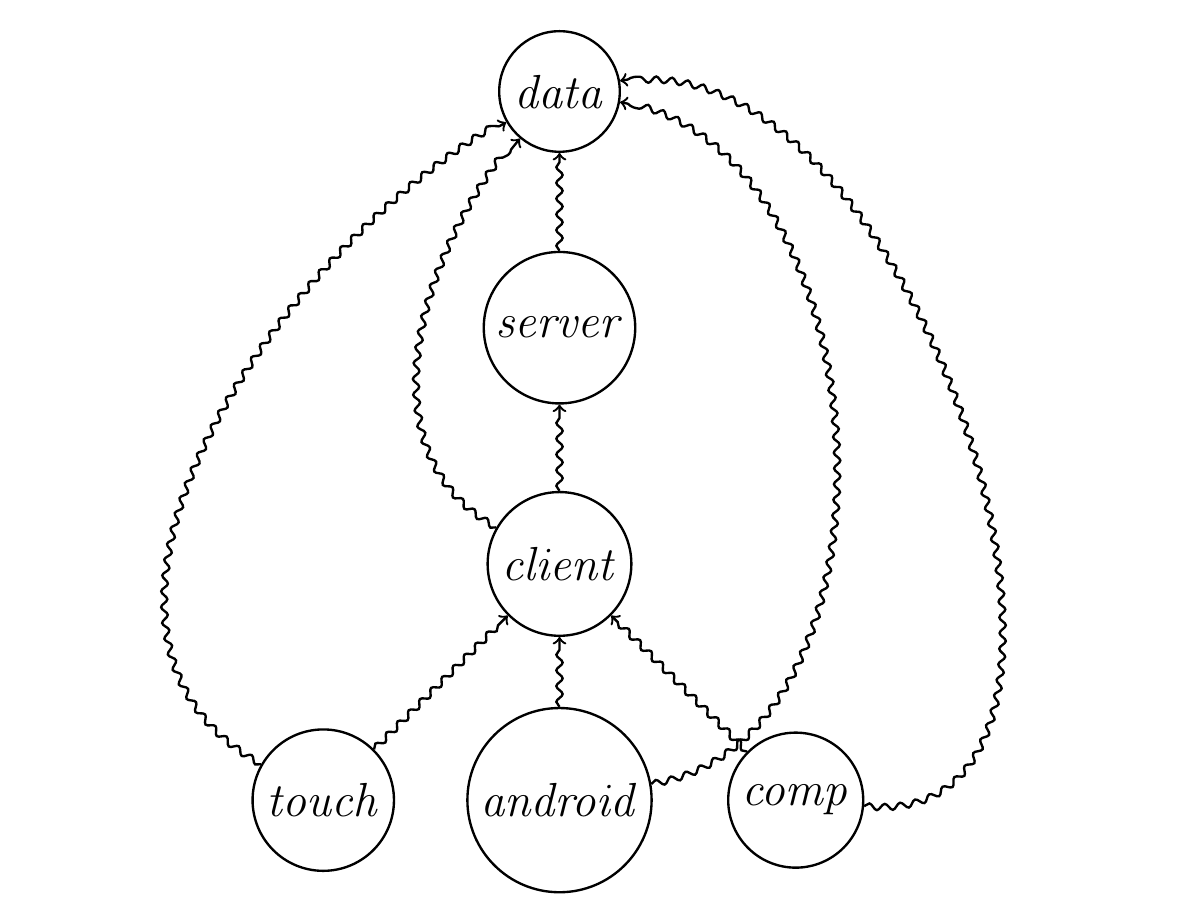
\begin{tikzpicture}
		\node (data) at (0,2) [shape=circle,line width=.3mm,draw] {\LARGE{\emph{data}}};
		\node (server) at (0,-1) [shape=circle,line width=.3mm,draw] {\LARGE{\emph{server}}};
		\node (client) at (0,-4) [shape=circle,line width=.3mm,draw] {\LARGE{\emph{client}}};
		\node (touch) at (-3, -7) [shape=circle,line width=.3mm,draw] {\LARGE{\emph{touch}}};
		\node (android) at (0, -7) [shape=circle,line width=.3mm,draw] {\LARGE{\emph{android}}};
		\node (comp) at (3, -7) [shape=circle,line width=.3mm,draw] {\LARGE{\emph{comp}}};
		\draw [->,line width=.3mm,decorate,
      decoration={snake,amplitude=.4mm,segment length=2mm,post length=1mm}] (server) -- (data);
		\draw [->,line width=.3mm,decorate,
      decoration={snake,amplitude=.4mm,segment length=2mm,post length=1mm}] (client) to[out=150, in=230] (data);
		\draw [->,line width=.3mm,decorate,
      decoration={snake,amplitude=.4mm,segment length=2mm,post length=1mm}] (client) -- (server);
		\draw [->,line width=.3mm,decorate,
      decoration={snake,amplitude=.4mm,segment length=2mm,post length=1mm}] (touch) -- (client);
		\draw [->,line width=.3mm,decorate,
      decoration={snake,amplitude=.4mm,segment length=2mm,post length=1mm}] (android) -- (client);
		\draw [->,line width=.3mm,decorate,
      decoration={snake,amplitude=.4mm,segment length=2mm,post length=1mm}] (comp) -- (client);
		\draw [->,line width=.3mm,decorate,
      decoration={snake,amplitude=.4mm,segment length=2mm,post length=1mm}] (touch) to[out=150, in=210] (data);
		\draw [->,line width=.3mm,decorate,
      decoration={snake,amplitude=.4mm,segment length=2mm,post length=1mm}] (android) to[out=10, in=-10] (data);
		\draw [->,line width=.3mm,decorate,
      decoration={snake,amplitude=.4mm,segment length=2mm,post length=1mm}] (comp) to[out=-5, in=10] (data);
	\end{tikzpicture}
	\caption{Graph diagram depicting the dependencies between modules in the project.}
\end{figure}
\end{document}